\chapter{Przykłady działania}
Platforma działała na urządzeniu Raspberry Pi 3B+.
W trakcie prac sterownik przekaźnikowy został podłączony za pomocą MQTT, który sterował lampką. Natomiast czujnik temperatury DS18B20 został podłączony bezpośrednio do portów GPIO od Raspberry. Płytkę Raspberry wykorzystano ze względu na: 
\begin{itemize}
    \item małe rozmiary, dzięki którym łatwiej znaleźć dedykowane stałe miejsce,
    \item małe zapotrzebowanie na energie, które ma bardzo duży wpływ w przypadku gdy urządzenie działa 24 godziny na dobę,
    \item mała cena, która wynosi ok 200 zł za wersje 3B+.
\end{itemize}
Oczywiście urządzenie to posiada dwie spore wady:
\begin{itemize}
    \item mała stabilność, która jest efektem tego, że system działa na karcie SD,
    \item do tego urządzenia należy samodzielnie dostarczyć zasilanie 5.1V o minimalnym natężeniu 2A. Często z winy słabej jakości kabla albo zasilacza awaryjność powoduje, że trzeba restartować urządzenie raz na miesiąc czy nawet na tydzień.
\end{itemize}
Warto jednak tutaj wspomnieć, że niektórzy miłośnicy Raspberry instalują system na dysku SSD, co znacznie wydłuża żywotność i przy lekkich platformach system potrafi pracować wiele lat bez przerwy spowodowanej awarią. Eliminuje to pierwszą wadę urządzenia lecz można się z tym raczej spotkać tylko w hobbistycznych projektach, a nie w komercyjnych rozwiązaniach.
\par
Wady i zalety pokazują, że jest to świetna konfiguracja prototypownia, a nie do długoterminowej instalacji. Jako, że grupa docelowa tej platformy głównie korzysta z tego urządzenia to postanowiono na nim stworzyć przykładową implementację.
\newpage
\section{Shelly}
Najbardziej kosztownym czasowo punktem było zintegrowanie platformy ze sterownikiem Shelly1, który może być sterowany przez protokół mqtt. \cite{mqtt, shelly}
\begin{figure}[h]
  \centering
  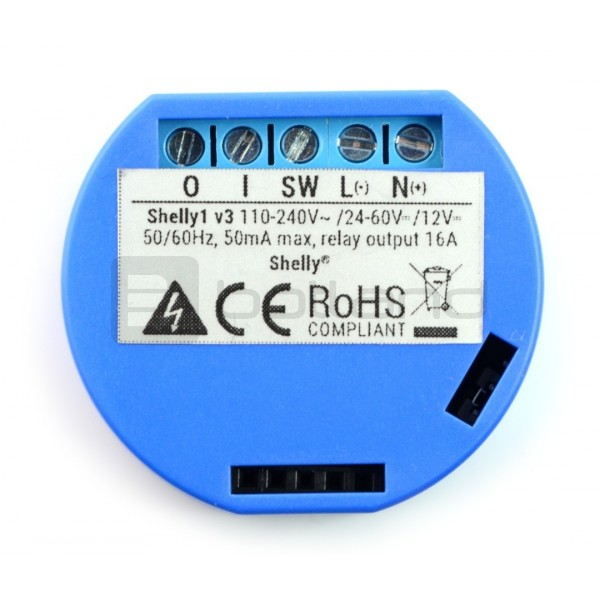
\includegraphics[width=\linewidth/2]{shelly1.jpg}
  \caption{Shelly1}
  \label{fig:shelly}
\end{figure}
API zostało udostępnione na stronie producenta i praca ta polegała na zintegrowaniu sterownika z serwerem.
API dla sterownika Shelly1 wygląda następująco:
\begin{itemize}
    \item shellies/<model>-<deviceid>/relay/0 by zaraportować \textit{on} lub \textit{off}
    \item shellies/<model>-<deviceid>/relay/0/command akceptuje \textit{on} lub \textit{off}
    \item shellies/<model>-<deviceid>/input/0 reportuje stan wejścia SW
    \item shellies/<model>-<deviceid>/longpush/0 reportuje stan długiego wciśnięcia jako 0 lub 1
\end{itemize}
dochodzi jeszcze jeden ogólny kanał dla każdego modelu \textit{shellies/announce} na którym "przedstawia się" każdy nowo podłączony sterownik.
\newpage
\begin{lstlisting}[columns=fullflexible,caption={sterowanie shelly}\label{lst:shelly},language=Java]
const shellies = {};
export const setRelay = (id, state) => {
	client.publish(`shellies/${id}/relay/0/command`, state);
};
const messageHandler = (deviceId, prop, message) => {
	if (shellies[deviceId] !== undefined) {
		shellies[deviceId][prop] = message;
		onDeviceChange({
			id: deviceId,
			...shellies[deviceId]
		});
	}
};
client.on('message', (topic, message) => {
	if (topic === 'shellies/announce') {
		const announcement = JSON.parse(message.toString());
		console.log('new shelly: ', announcement.id);
		shellies[announcement.id] = { ip: announcement.ip };
	} else {
		const id = topic.split('/')[1];
		const prop = topic.split('/')[2];
		messageHandler(id, prop, message.toString());
	}
});
\end{lstlisting}
\section{DS18B20}
DS18B20 to termometr cyfrowy obsługiwany przez protokół 1-wire. W przedstawionej implementacji jest on podłączony w trybie \textit{paraside} na dwie żyły gdzie jedna to masa, a druga jest jednocześnie zasilaniem jak i linią danych. 
\par Implementacja jest znacznie łatwiejsza niż w przypadku Shelly, ponieważ ogranicza się do pobrania modułu \textit{ds18b20-raspi} z repozytorium npm i skonfigurowania wyjść Raspberry. \par
Konfiguracja ogranicza się do włączeniu obsługi interface'u 1-wire w ustawieniach urządzenia. Czujnik został podłączony do domyślnego portu, którym jest GPIO4. Efekt końcowy widać na zdjęciu \ref{fig:finalGPIOConnections} \cite{linux}
\par Można odczytać wartość pomiaru przy użyciu jednej funkcji w 2 wariantach: synchronicznej \ref{lst:ds18b20sync} i asynchronicznej \ref{lst:ds18b20async}. Moduł exportuje funkcję \textit{readDataWithInterval}, która odczytuje wartość co 30 sekund. Skraca to implementację w module głównym.
\newpage
\begin{lstlisting}[columns=fullflexible,caption={ds18b20.js}\label{lst:ds18b20},language=Java]
import sensor from 'ds18b20-raspi'
const intervalsId = [];

export const readTemp = (id) => {
    return new Promise((resolve, reject) => {
        sensor.readC(id, 2, (err, temp) => { /*!\annotation{lst:ds18b20async}!*/
            if (err) {
                reject(err)
            } else {
                resolve(temp);
            }
        })
    })
}

export const readDataWithInterval = (id, callback) => {
    intervalsId.push(setInterval(() => {
        const temp = sensor.readC(id) /*!\annotation{lst:ds18b20sync}!*/
        callback(temp, id);
    }, 30000))
}

export const clearAllTasks = () => {
    intervalsId.forEach(intervalId => clearInterval(intervalId))
}
\end{lstlisting}
\begin{figure}[h]
  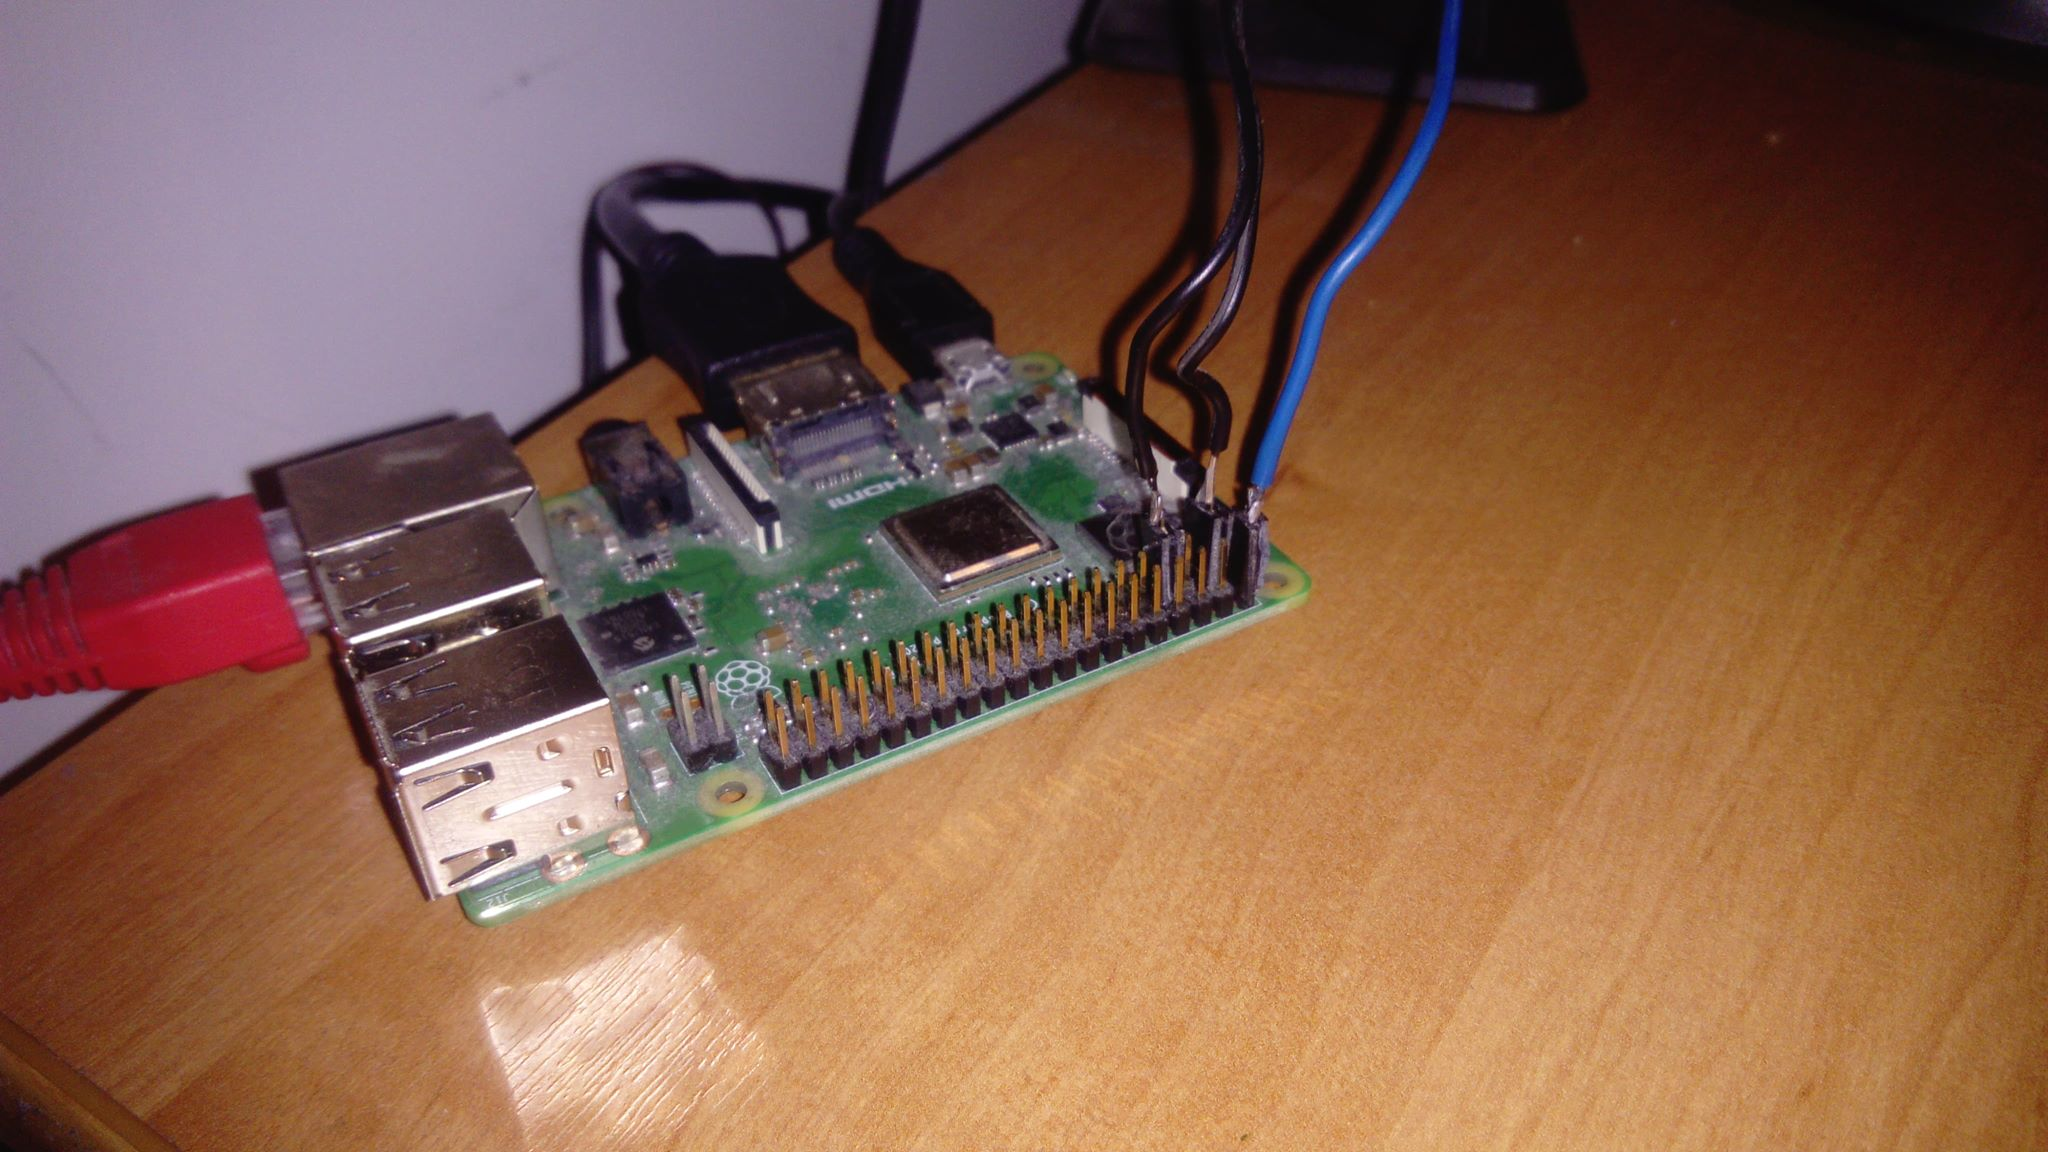
\includegraphics[width=\linewidth]{gpio.jpg}
  \caption{podłączenie czujnika DS18B20}
  \label{fig:finalGPIOConnections}
\end{figure}